\chapter{初识Slam}

\begin{figure}[!htbp]
    \centering
    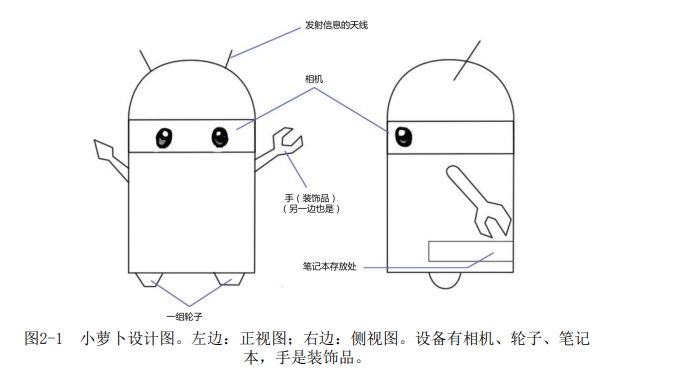
\includegraphics[width=0.6\textwidth]{image/chapter01/小萝卜机器人.png}
    \caption{小萝卜机器人设计图}
\end{figure}

    以小萝卜为例,我们希望小萝卜具有自主运动能力,那么对应的,我们就应该对小萝卜的设计有一定的要求

\begin{itemize}
    \item [1)] 首先,移动需要有\emph{轮子和电机}  
    \item [2)] 其次,如果光有移动能力但不知道行动的目标也是不行的。为了避免这种情况,我们需要一个\emph{相机以充当眼睛}
    \item [3)] 然后还要有\emph{接受信息的天线}
\end{itemize}

    那么,为了能够让小萝卜在\emph{能够在任意环境中轻松自在地行走,我们至少需要让他知道}:

    \begin{itemize}
        \item [-] 定位:我在什么地方?
        \item [-] 建图:周围环境是什么样?
    \end{itemize}

\section{传感器}

\begin{quote}
    \centering
    定位和建图可以看作感知的“内外之分”。
\end{quote}

    一类传感器是携带于机器人本体上的:\emph{携带于本体上的传感器没有对环境提出任何要求,从而使得这种方案可适用于未知环境}; 另一类传感器是安装于环境中的:\emph{安装于环境中的传感设备,通常能够简单有效地解决定位问题,但是必须要在一定的环境中,从而限制了机器人的适用范围}。

    值得注意的是:\emph{Slam非常强调未知环境},因此通常我们都是通过相机来完成Slam

    相机的种类是多种的,Slam中使用的相机与平时简单的单反摄像头并不一样。而\emph{照片的本质是拍照时的场景(Scene)在相机的成像平面上留下的一个投影。它以二维的形式反映了三维的世界}。那么显然的,这个过程中丢掉了一个维度:\emph{深度(距离)}

\subsection{单目相机}

\begin{quote}
    \centering
    只使用一个摄像头进行Slam的做法称为\emph{单目Slam}。
\end{quote}

这种传感器结构简单,成本较低。但是,由于\emph{单目相机拍摄的图像只是三维空间中的二维投影,所以丢失深度的单目需要改变相机的视角,才能估计到运动(Motion)的发生,同时估计场景中物体的远近和大小,不妨称之为结构(Structure)}。通过\emph{近处的物体移动快,远处则慢}这一原理,使得物体在图像上的运动形成了\emph{视差},就能够获取一个相对的深度

因此,单目Slam估计的轨迹和地图将与真实的轨迹和地图相差一个因子,被称为\emph{尺度(Scale)},又称为\emph{尺度不确定性}。

\begin{figure}[!htbp]
    \centering
    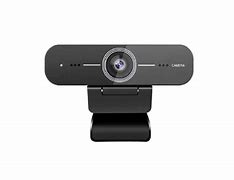
\includegraphics[width=0.6\textwidth]{image/chapter01/单目相机.jpg}
    \caption{单目相机示意图}
\end{figure}

\subsection{双目相机}

\begin{quote}
    \centering
    双目相机由两个单目相机组成,但这两个相机之间的距离(被称为基线)时已知的
\end{quote}

类似于人眼一样,通过左右眼图像的差异判断物体的远近。\emph{计算机上的双目相机需要大量计算才能(不太可靠的)估计每一个像素点的深度。双目相机测量到的深度范围与基线相关。基线越大,能够测量到的范围越远}。但是,双目或夺目相机的缺点时配置与标定均为复杂,其深度量程和精度受双目相机的基线和分辨率所限,且计算非常消耗计算机资源。

\begin{figure}[!htbp]
    \centering
    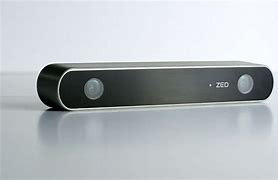
\includegraphics[width=0.6\textwidth]{image/chapter01/双目相机.jpg}
    \caption{双目相机示意图}
\end{figure}

\subsection{深度相机(RGB-D)}

\begin{quote}
    \centering
    深度相机可以通过\emph{红外结构光或者 $Time-of-Flight(TOF)$ 原理,通过主动向物体发射光并接受返回的光,从而测量物体与相机之间的距离}
\end{quote}

    深度相机通过\emph{物理的测量手段},所以对比于双目相机可以节省大量的计算。但是,目前的RGB-D相机还存在\emph{测量范围窄、噪声大、视野小、易受日光干扰、无法测量投射材质等诸多问题}。

\begin{figure}[!htbp]
    \centering
    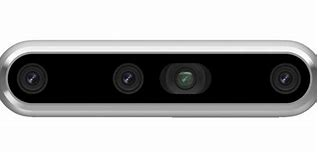
\includegraphics[width=0.6\textwidth]{image/chapter01/深度相机.jpg}
    \caption{深度相机示意图}
\end{figure}

\section{经典视觉Slam框架}

\begin{figure}[!htbp]
    \centering
    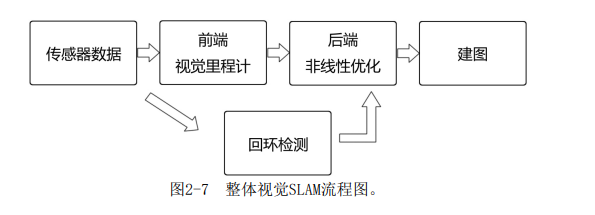
\includegraphics[width=0.4\textwidth]{image/chapter01/视觉Slam框架.png}
    \caption{经典视觉Slam框架}
\end{figure}

    \emph{经典的视觉Slam框架本身和所包含的算法基本已经定型},整个视觉Slam的流程为:

\begin{itemize}
    \item [1)] 传感器信息读取:在视觉中主要以相机图像信息的读取和预处理
    \item [2)] 视觉里程计($Visual Odometry, VO$):视觉里程计的任务时估算相邻图像间相机的运动,以及局部地图的样子,又被称为前端($Front End$)
    \item [3)] 后端优化($Optimization$):后端接受不同时刻视觉里程计测量的相机位姿,以及回环检测的信息,对它们进行优化,得到全局一致的轨迹和地图,又称为后端($Back End$)
    \item [4)] 回环检测($Loop Closing$):回环检测判断机器人是否达到过先前的位置,如果检测到回环,把信息提供给后端进行处理
    \item [5)] 建图($Mapping$):根据估计的轨迹,建立与任务要求对应的地图
\end{itemize}

\subsection{视觉里程计}

\begin{quote}
    \centering
    视觉里程计关心的时\emph{相邻图像之间的相机运动}
\end{quote}

    如果用人眼来说,我们很轻易就知道我们是否发生移动,是否发生旋转,但是在相机中,我们能够知道发生了旋转,但是\emph{我们具体旋转了多少度,平移了多少里面,我们就很难给出确切答案了}。
    
    那么,我们需要知道\emph{相机与空间点的几何关系以及$VO$的实现方法(在后续介绍)}。$VO$能够通过相邻帧的图像估计相机运动,并恢复场景的空间结构。$VO$之所以叫做里程计,是因为其和实际的里程计一样,\emph{只计算相邻时刻的运动,而和过往的信息没有关联}。
    
\begin{figure}[!htbp]
    \centering
    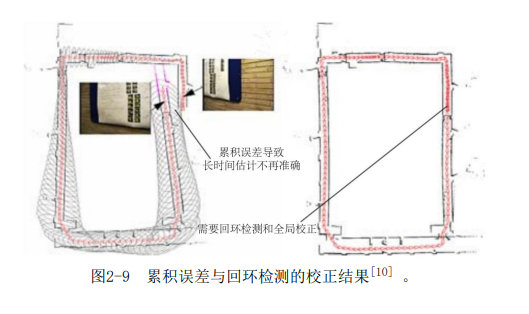
\includegraphics[width=0.6\textwidth]{image/chapter01/回环误差.png}
    \caption{VO出现累积漂移}
\end{figure}

    当然,仅仅通过视觉里程计来估计轨迹,将不可避免的出现\emph{累计漂移(Accumulating Drift)}。\emph{这是由于视觉里程计只估计两个图像之间的运动造成的,而每一次的估计都会有一定的误差,误差不断传递并累计造成了漂移(Drift)}。为了解决漂移问题,引入后续两种技术:\emph{后端优化和回环检测}。

\subsection{后端优化}

\begin{quote}
    \centering
    笼统的说,后端优化主要指处理Slam过程中噪声的问题。
\end{quote}

    对于实际来说,不管多么精确的传感器都有一定的误差,后端要考虑的问题,就是\emph{如何从这些带有噪声的数据库中估计整体系统的状态,以及这个状态估计的不确定性有多大},这被称为最大后验概率估计($Maximum-a-Posterioru, MAP$)。这里的状态既包括自身的轨迹,也包括地图。\emph{在视觉Slam中,前端和计算机视觉领域研究更为相关}。
    
    Slam问题的本质为:\emph{对运动主体自身和周围环境空间不确定性的估计},为了解决Slam问题,我们需要\emph{状态估计理论把定位和建图的不确定性表达出来,然后采用滤波器或非线性优化,估计状态的均值和不确定性(在后续介绍)}。

\subsection{回环检测}

\begin{quote}
    \centering
    回环检测又称闭环检测($Loop Closure Detection$),主要解决\emph{位置估计随时间漂移}的问题
\end{quote}

    假设实际情况下机器人经过一段时间后回到原点,由于漂移,它的位置估计值却没有回到原点,通过某种手段让机器人知道回到原点。
    
    回环检测与定位和建图有密切的关系,事实上,我们更希望机器人自身判断图像间的相似性。

\subsection{建图}

\begin{quote}
    \centering
    建图($Mapping$)是指构建地图的过程。地图是对环境的描述,但是该描述是不固定的
\end{quote}

\begin{figure}[!htbp]
    \centering
    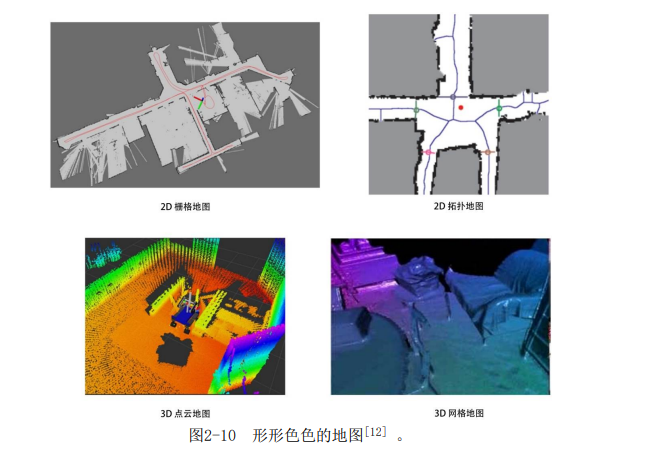
\includegraphics[width=0.4\textwidth]{image/chapter01/建图示意.png}
    \caption{建图示意图}    
\end{figure}

    \textbf{度量地图(Metric Map)},度量地图\emph{强调精确地表示地图中物体的位置关系,通常用稀疏($Sparse$)与稠密($Dense$)对其分类}

    稀疏地图进行了一定程度的抽象,并不需要表达所有的物体。我们可以选择一部分具有代表意义的东西,称为路标($Landmark$),然后只记录路标即可。稀疏地图常用于定位,但是对于导航来说,需要使用稠密地图。

    \textbf{拓扑地图($Topological Map$)},拓扑地图\emph{更强调地图元素之间的关系}。拓扑地图是一个图($Graph$),由节点和边组成,只考虑节点之间的连通性。它放松了地图对精确位置的需要,去掉了地图的细节问题。

\section{Slam问题的数学表达}

\begin{quote}
    \centering
    假设小萝卜正携带某种传感器在未知环境里运动,怎么用数学语言描述?
\end{quote}

    由于相机通常是在某些时刻采集数据的,所以我们只关心这些时刻的位置和地图:
\begin{itemize}
    \item [1)] 记离散时刻为:$t = 1, \dots, K$
    \item [2)] 用$x$表示小萝卜自身的位置,于是:$x_1, \dots, X_K$表示各时刻的位置,构成了小萝卜的轨迹
    \item [3)] 地图中,假设地图是由多个路标组成的,而每个时刻都会测量到一部分路标,设路标点一共有$N$个,用$y_1, \dots, y_N$表示
\end{itemize}

    什么是运动,我们要考虑从$K - 1$时刻到$K$时刻,小萝卜的位置$x$是如何变化的

    通常,机器人会携带一个测量自身运动的传感器,那么我们可以抽离出一个通用数学模型

$$
    x_k = f(x_{k - 1}, u_k, w_k)
$$

    这里,$U_k$是运动传感器的读数(也叫做输入),$W_k$为噪声。我们使用函数$f$来指代任意的运动传感器,称为运动方程。
    
    什么是观测,假设小萝卜在$k$时刻于$X_k$处探测到某一个路标$y_j$,我们需要考虑如何用数学语言描述:

    与运动方程对应的,还有一个观测方程。观测方程描述的是,当小萝卜在$X_k$位置上看到的某个路标点$y_j$,产生了一个观测数据$Z_{k,j}$。用抽象函数$h$来描述:

$$
    Z_{k, j} = h(y_j, x_k, v_{k, j})
$$

    这里,$V_{k, j}$是这次观测里的噪声,为了保证通用性,将其取为抽象形式,则可总结为两个基本方程

$$
\begin{cases}
	x_k = f(x_{k - 1}, u_k, w_k) \\
	z_{k,j} = h(y_j, x_k, v_{k, j})
\end{cases}
$$

